\section{Unconstrained Programming Exercices}

\subsection{Problem 1}

Discutez, suivant les valeurs du paramètre $\beta \in \mathrm{R}$, la nature des points stationnaires de la fonction de deux variables
\[
f(x,y) = x^2 + y^2 + \beta xy + x + 2y
\]

\textbf{Answer}
\begin{align*}
\nabla f(x,y) &= 
	\begin{bmatrix}
		2x + \beta y + 1 \\
		2y + \beta x + 2
	\end{bmatrix} \\
\textbf{H}(f(x,y)) &=
	\begin{bmatrix}
		2 & \beta \\
		\beta & 2
	\end{bmatrix}
\end{align*}
Find the eigen values
\begin{align*}
\text{det}(\lambda I - \textbf{H}) &= 0 \\
\text{det}\Bigg( 
	\begin{bmatrix}
		\lambda -2 & -\beta \\
		-\beta & \lambda - 2
	\end{bmatrix}
\Bigg) &= 0 \\
(\lambda -2)^2 - \beta^2 &= 0 \\
\lambda^2 -4\lambda + y - \beta^2 &= 0
\end{align*}
Using the quadratic formula
\begin{align*}
\lambda &= \frac{4 \pm \sqrt{16 - 4 \cdot 1 \cdot (4-\beta^2)}}{2} \\
&= \frac{4 \pm \sqrt{4 \beta^2}}{2} \\
&= \frac{4 \pm 2\beta}{2} \\
&= 2 \pm \beta
\end{align*}

\begin{center}
\begin{tabular}{|c|c|c|}
	\hline
	$\beta < -2$ & $\beta \in [-2, 2]$ & $\beta > 2$ \\
	\hline
	$\lambda_1 < 0$, $\lambda_2 > 0$ & $\lambda_1 = [0, 4]$, $\lambda_2 = [4, 0]$& $\lambda_1 > 0$, $\lambda_2 < 0$\\
	Indefinite matrix & Semi-definite positive matrix & Indefinite matrix\\
	\hline
	Saddle point & local minimum & saddle point \\
	\hline
\end{tabular}
\end{center}

\pagebreak
\subsection{Problem 2}

Soit la minimisation sans contraintes de la fonction
\[
f(x_1,x_2) = 2x_1^2 + x_2^2 -2x_1x_2 + 2x_1^3 + x_1^4
\]
\begin{enumerate}[(a)]
\item Trouvez les candidats solution du problème et pour chacun d’entre eux, précisez s’il s’agit d’un minimum local, d’un maximum local ou d’un point selle. Justifiez vos réponses.
\item Y a-t-il un minimum global dans ce cas? Si oui, lequel?
\end{enumerate}

\textbf{Answer}

\textbf{a)}
\begin{align*}
\nabla f(x_1, x_2) =
\begin{bmatrix}
4x_1 - 2x_2 + 6x_1^2 + 4x_1^3 \\
2x_2 - 2x_1
\end{bmatrix} &= 0\\
2x_2 - 2x_1 &\Rightarrow x_2 = x_1
\end{align*}
Substituting into the first line we get
\begin{align*}
	4x_1^3 + 6x_1^2 + 2x_1 &= 0 \\
	2x_1^3 + 3x_1^2 + x_1 &= 0 \\
	x_1(2x_1+1)(x_1+1) &=0 \\
	x_1 = 0, -1 \text{ or } -\frac{1}{2}
\end{align*}
Our 3 stationary points are $(0,0)$, $(-1,-1)$ and $(-\frac{1}{2}, -\frac{1}{2})$
\begin{align*}
\textbf{H} = 
\begin{bmatrix}
	12x_1^2 + 12x_1 + 4 & -2 \\
	-2 & 2
\end{bmatrix}
\end{align*}
Find the eigen values of the hessian
\begin{align*}
\text{det}(\lambda I - \textbf{H}) &= 0 \\
\text{det}\Bigg( 
\begin{bmatrix}
	\lambda -4(3x_1^2 + 3 x_1 + 1) & -2 \\
	-2 & \lambda -2
\end{bmatrix}
\Bigg) &= 0 \\
\Big(\lambda -4(3x_1^2 + 3 x_1 + 1)\Big)(\lambda -2) -4 &= 0
\end{align*}
For $(x_1, x_2) = (0,0)$ we have
\begin{align*}
	(\lambda-4(0-0+1))(\lambda -2 ) -4 &= 0 \\
	(\lambda -4)(\lambda -2) -4 &= 0 \\
	\lambda^2 - 6\lambda + 4 &= 0 \\
	\lambda &= \frac{6 \pm \sqrt{36 - 4 \cdot 4}}{2} \\
	\lambda &= 3 \pm \sqrt{5} \\
	\lambda_1 > 0, \lambda_2 >0
\end{align*}
Both values of $\lambda$ are positive making the Hessian definite positive at $(0,0)$ making the point a local minimum.

For $(x_1, x_2) = (1,1)$ we have
\begin{align*}
(\lambda-4(3-3+1))(\lambda -2 ) -4 &= 0 \\
(\lambda -4)(\lambda -2) -4 &= 0
\end{align*}
Which goes back to the same answer as above, thus $(1,1)$ is also a local minimum.

For $(x_1, x_2) = (-\frac{1}{2},-\frac{1}{2})$ we have
\begin{align*}
(\lambda-4(-\frac{3}{4} - \frac{6}{4} + \frac{4}{4}))(\lambda -2 ) -4 &= 0 \\
(\lambda +5)(\lambda -2) -4 &= 0 \\
\lambda^2 + 3 \lambda -14 &= 0 \\
\lambda &= \frac{-3 \pm \sqrt{9-4 \cdot 1 \cdot -14}}{2} \\
\lambda &= \frac{-3 \pm \sqrt{65}}{2}
\lambda &= 2.5311, -5.5311
\end{align*}
Meaning the Hessian is indefinite at $(-\frac{1}{2},-\frac{1}{2})$ making it a saddle point.

\subsection{Problem 3}

On dit qu’un ensemble $C \subseteq \mathrm{R}^n$ est convexe si
\[
	\lambda x+(1-\lambda )y \in C\ \ \ \forall \lambda \in [0,1],\ x, y \in C
\]

\textbf{a)} Donnez une interprétation géométrique de cette propriété et tracez un sous-ensemble de $\mathrm{R}^2$ qui n’est pas convexe.

\answer

We have two points $x$ and $y$ in $C$. If we draw a line from $x$ to $y$, the entire line has to always stay in $C$.
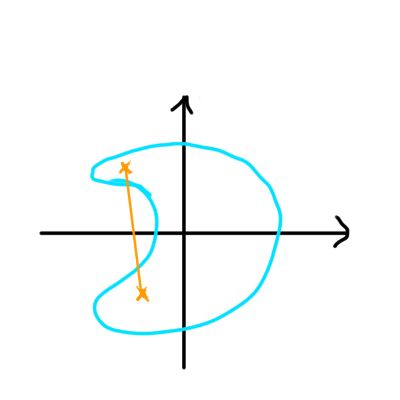
\includegraphics[scale=0.5]{fig/unconstrained_exercices/pb3a.jpg}

\pagebreak
\textbf{b)} 

\answer\footnote{\url{http://ljk.imag.fr/membres/Anatoli.Iouditski/cours/convex/chapitre_3.pdf} page 57}

Let $x,\ y\ \in C_\alpha$, take $f$ of the convex equation
\begin{align*}
f\Big(\lambda x + (1-\lambda)y \Big) &\geq f(\lambda x) + f\Big((1-\lambda)y\Big)
\intertext{Since $f$ is convex we can write by definition that}
f(\lambda x + (1-\lambda)y) &\geq f(\lambda x) + f((1-\lambda)y) \geq \lambda f(x) + (1-\lambda)f(y)
\end{align*}
Since  $x,\ y\ \in C_\alpha$ we can write
\[
f(\lambda x + (1-\lambda)y) \geq \lambda \alpha + (1-\lambda) \alpha
\]
Which is the same as
\[
f(\lambda x + (1-\lambda)y) \geq \alpha
\]
Thus $C_\alpha$ is convex
\textbf{c)}

\answer

The epigraph is the volume on top of a curve, including the curve itself. So we choose two points $(x_1, t_1)$ and $(x_2, t_2)$ both $\in \text{epi}(f)$ meaning that
\begin{align*}
	f(x_1) &\leq t_1 \\
	f(x_2) &\leq t_2
\end{align*}
To show that epi$(f)$ is convex we need to show that
\[
\lambda(x_1, t_1) + (1-\lambda)(x_2,t_2) \in \text{epi}(f)
\]
We can rewrite the lhs as the point
\[
\Big(\lambda x_1 + (1-\lambda) x_2,\ \lambda t_1 + (1-\lambda) t_2\Big) \in \text{epi}(f)
\]
which would mean that the value of $f$ from $x_1$ to $x_2$ should be less than the line $t_1$ to $t_2$ for any $\lambda \in [0, 1]$ i.e.
\[
f(\lambda x_1 + (1-\lambda) x_2) \overset{?}{\leq} \lambda t_1 + (1-\lambda) t_2
\]
Since $f$ is convex we can write
\[
f(\lambda x_1 + (1-\lambda) x_2) \leq\ \lambda f(x_1) + (1-\lambda)f(x_2) \ \leq \lambda t_1 + (1-\lambda) t_2
\]
which means the previous equation is true, thus epi$(f)$ is convex.

\textbf{d)}

\answer

We want to show that for two points $x_1,\ x_2 \in M$ we have
\[
\lambda x_1 + (1-\lambda)x_2 \in M
\]
We can do this by showing that the linear combination of $x_1$ and $x_2$ is still a minimum of $f$.
\[
f(\lambda x_1 + (1-\lambda)x_2) \overset{?}{\leq} f(x)\ \ \ \ \forall x
\]
Since $f$ is convex we can write
\[
\lambda f(x_1) + (1-\lambda)f(x_2) \overset{?}{\leq} f(x)
\]
But since $x_1$ and $x_2$ are both global minima of $f$ then $f(x_1) = f(x_2)$ and we can write
\begin{align*}
\big(\lambda + (1-\lambda)\big)f(x_1) &\overset{?}{\leq} f(x) \\
f(x_1) &\overset{?}{\leq} f(x)
\end{align*}
Which is true since we know $x_1$ is a global minimum. Thus the set $M$ is convex.

\textbf{e)}

\answer








